%==============================================================================
% SBR/LARS 2026 (Robotica 2026, Joao Pessoa) — Conference paper (6 pages, IEEE)
% DOUBLE-BLIND submission. Template: IEEEtran (conference).
%
% STATUS: SKELETON + SAFE SECTIONS. Method and Results are written from validated
% repository artifacts; Introduction / Related Work / Discussion / Limitations /
% Abstract are structured STUBS with explicit TODOs (see each file).
%
% BASELINE NAMING: the comparison baseline is rSim (the ODE physics engine of the
% rSoccer environment) — NOT grSim. Use "rSim" everywhere. The first mention in
% the text spells out what it is.
%
% Build: pdflatex main && bibtex main && pdflatex main && pdflatex main
% (References render once refs/references.bib is populated by the focused review.)
%==============================================================================
\documentclass[conference,a4paper]{IEEEtran}
\IEEEoverridecommandlockouts
\usepackage{cite}
\usepackage{amsmath,amssymb,amsfonts}
\usepackage{graphicx}
\usepackage{textcomp}
\usepackage{xcolor}
\usepackage{booktabs}
\usepackage{siunitx}
\usepackage{url}
\usepackage{tikz}
\usetikzlibrary{arrows.meta,positioning,fit,backgrounds,calc}
\usepackage{stfloats}   % permite figure*/table* no rodapé; evita floats empurrados
                        % para depois das referências (falha observada em 2026-08-07)
\graphicspath{{figures/}}

% --- Float placement -----------------------------------------------------
% O build de 2026-08-07 empurrou Fig.2 e Fig.3 para DUAS páginas órfãs depois
% das referências (8 floats: 3 figuras + 5 tabelas). Os defaults do LaTeX
% (topnumber=2, totalnumber=3, textfraction=0.2) são restritivos demais aqui.
\setcounter{topnumber}{3}
\setcounter{bottomnumber}{2}
\setcounter{totalnumber}{4}
\renewcommand{\topfraction}{0.92}
\renewcommand{\bottomfraction}{0.85}
\renewcommand{\textfraction}{0.07}
\renewcommand{\floatpagefraction}{0.70}

% --- Pending-number marker (REGRA DE OURO) ---------------------------------
% Every number that enters the paper must come from a repository artifact.
% Where a number is required but does not yet exist, \TODO{origin} marks it and
% the exact command that produces it is registered in docs/TASKS_CLAUDE_CODE.md.
% MUST be empty (zero occurrences) before submission.
\newcommand{\TODO}[1]{\textcolor{red}{\textbf{[TODO: #1]}}}
\def\BibTeX{{\rm B\kern-.05em{\sc i\kern-.025em b}\kern-.08em
    T\kern-.1667em\lower.7ex\hbox{E}\kern-.125emX}}

% --- Notation shortcuts -------------------------------------------------------
\newcommand{\epos}{e_{\mathrm{pos}}}
\newcommand{\eang}{e_{\mathrm{ang}}}
\newcommand{\SEtwo}{\mathrm{SE}(2)}
\newcommand{\Td}{T_{d}}

\begin{document}

%------------------------------------------------------------------------------
% DOUBLE-BLIND TITLE/AUTHOR BLOCK (anonymization checklist A1,A2,A9,A10).
% No names, no affiliation, no funding, no ORCID until camera-ready.
%------------------------------------------------------------------------------
% --- Title decision (2026-07-31, redação): the previous title ("... from
% Closed-Loop Competition Logs ...") stated the inverse of the central finding
% (yaw is identified from a DEDICATED OPEN-LOOP collection precisely because
% closed-loop logs fail). Three regime-aware alternatives were considered;
% the first is applied below. The other two, kept for the record:
% Alt 2: When Competition Logs Are Not Enough: Excitation-Dependent
%        Identifiability in a Per-DOF Digital Twin of an Omnidirectional
%        Soccer Robot
% Alt 3: Per-DOF Grey-Box Digital Twinning of an Omnidirectional Soccer
%        Robot: Multi-Horizon Fidelity and Identifiability Across Excitation
%        Regimes
% --- Title revision (2026-08-07, revisão maior) -------------------------------
% Hybrid form approved by the author: keeps the reality-gap framing requested in
% the revision brief (T1) AND the central finding that the 2026-07-31 decision
% was built on. The literal T1 title ("A Behavioral Model for Reality-Gap
% Mitigation in Digital Twins of Omnidirectional Soccer Robots") was NOT applied
% verbatim: it drops the identifiability result and promises a gap-mitigation
% claim that is validated only on translation-dominated windows against an
% untuned rSim (reviewer B5). Deviation registered in docs/REGISTRO_DESVIOS.md.
% 2026-08-10: título trocado por decisão do autor após a revisão independente.
% O anterior ("A Behavioral Model for Reality-Gap Mitigation in Digital Twins of
% Omnidirectional Soccer Robots") prometia MITIGAÇÃO do reality gap, que é uma
% alegação sobre transferência: nenhuma política é treinada nem transferida aqui
% (bloqueador B5). O novo título nomeia o que o artigo de fato mede.
% AÇÃO DO AUTOR: atualizar o registro preliminar no JEMS.
% 2026-08-10 (3a volta, decisao do autor): removido "for Reality-Gap Mitigation",
% que prometia transferencia (treinar e transferir politica) -- algo que o artigo
% NAO mede, apontado por tres revisoes independentes. O reality gap permanece
% como MOTIVACAO na Introducao, onde e legitimo. O subtitulo nomeia a
% contribuicao de fato entregue. AÇÃO: atualizar o registro no JEMS.
\title{A Behavioral Model for Digital Twins of Omnidirectional Soccer Robots:
Diagnosing Identifiability from Competition Logs}

\author{\IEEEauthorblockN{Anonymous Author(s)}
\IEEEauthorblockA{\textit{Affiliation withheld for double-blind review}}}

\maketitle

%==============================================================================
% ABSTRACT — reposicionado 2026-08-10 apos a revisao independente.
% Mudancas:
%  - comparador PRIMARIO passa a ser a cinematica ideal (mesmo harness, mesma
%    inicializacao). rSim vira contexto, com a ressalva fitted-vs-untuned (B2/B3).
%  - estatistica reportada por EVENTO (n=10), nao por janela (item 9 / C11).
%  - acrescentadas as tres omissoes que o revisor cobrou (6.3): heading pior em
%    horizonte longo, 99.6% da validacao e translacional, rSim nao sintonizado.
%  - declarado o tamanho da evidencia em segundos (C11).
% IEEE: sem simbolos matematicos, sem citacoes. ~215 palavras.
% Numeros: 87% (CHANGELOG 2026-06-14); 71.1% (identificacao_omega_20260724.md);
% 1% (omega_excitation_analysis_20260807_133917.json); 0.038/0.101 e
% decomposicao (gap_decomposition_20260809_2308.md); p e efeito por evento
% (clustered_stats_20260809_2309.md); 73.5 s idem.
%
% REVISAO 2026-08-10 (pedido do autor), tres mudancas:
%  1. ABLACAO reescrita em linguagem plana: "switch each ingredient off in every
%     combination" em vez de "order-independent ablation". Mesmo conteudo
%     (Shapley sobre o fatorial 2^3, tau 55% / Td 43% / K 2%), sem o jargao.
%     Acrescentado o 0.114 m do braco "from rest", que torna o achado de
%     interacao verificavel em vez de assertivo.
%  2. rSim EXPLICITO e com resultado: 0.129 m em h_ref, nomeado, na mesma frase
%     do modelo e da cinematica ideal. Ressalva fitted-vs-untuned MANTIDA (B5) e
%     a ablacao de atraso casado entra como evidencia. O elo "roda do repouso,
%     como o rSim" liga a ablacao ao resultado do rSim -- explica o numero em vez
%     de so reporta-lo.
%  3. REMOVIDA a frase dos 99.6% translacional. ATENCAO: era uma das tres
%     omissoes que o revisor independente cobrou (item 6.3). A limitacao
%     PERMANECE enunciada em 06_limitations.tex, paragrafo "Evaluation and
%     scope", primeira frase. Se o revisor reabrir o ponto, a resposta e essa.
%
% Custo: ~240 -> ~270 palavras. Fonte dos numeros novos: 0.129 e 0.114 de
% results/epos_eang_three_models_20260810_1022.md (execucao canonica, mesma da
% Tabela III e da Fig. 2); atraso casado de
% results/eval_rsim_delay_ablation_20260809_2154.md.
%
% PENDENTE (nao aprovado pelo autor): o par 0.039/0.101 e mediana POR JANELA
% (gap_decomposition), enquanto "ten hold-out events" e por EVENTO
% (clustered_stats: 0.0421 vs 0.1177, gap +0.0689). A frase mistura as duas
% unidades. Mantido como estava ate decisao.
%==============================================================================
\begin{abstract}
Teams in the RoboCup Small Size League validate control software largely in
simulation, whose simplified physics leaves a reality gap to the field. This
paper asks what a behavioral model of an omnidirectional soccer robot can be
identified from the competition logs teams already record, and what those logs
cannot supply. Modeling each degree of freedom as one first-order channel with
dead time, the translational channels identify directly from in-game logs and
reach roughly 87 percent hold-out fit. The yaw channel does not: in play the yaw
command is a median of one percent of what the four wheels are asked to do, and
explains only 56 percent of the variance of the measured rotation, against 94 to
96 percent for translation. A short dedicated open-loop campaign restores the
excitation and identifies the channel at 71 percent hold-out fit. Fidelity is
then evaluated in free run over horizons from 0.1 to 1.5 seconds, every plant
under an identical harness. Over 73.5 seconds of scored motion the model reaches
0.039 metre of median position error at the 0.4-second horizon, against 0.101
for ideal kinematics and 0.129 for rSim, the ODE simulator used across the
league; all ten hold-out events favor the model. Switching each ingredient off
in every combination, so the attribution does not depend on removal order, the
lag in reaching commanded speed and the dead time before the robot responds
contribute in comparable parts, and the fitted gain almost nothing. The
improvement also requires starting each window from the measured velocity: from
rest the model gives 0.114 metre and no longer beats ideal kinematics, which is
how rSim runs for want of a velocity setter. Since rSim also runs at default
parameters against a plant fitted to this robot, and giving it the model's dead
time widens the difference rather than closing it, we report that comparison as
context, not as a general dynamical advantage.
\end{abstract}


\begin{IEEEkeywords}
digital twin, system identification, grey-box modeling, omnidirectional robot,
robot soccer, excitation design, fidelity evaluation
% FIX 2026-08-10: "sim-to-real" removido das keywords -- nenhuma transferencia
% e feita no artigo (opcional (i) da revisao V2). Trocado por "excitation design".
\end{IEEEkeywords}

%==============================================================================
% INTRODUCTION — corte 9->6 paginas (2026-08-10, pedido do autor).
%  - 4o paragrafo ("This paper models...") REMOVIDO: repetia o abstract e as
%    contribuicoes. O essencial (o que e medido, contra o que) migrou para uma
%    frase de fecho do 3o paragrafo.
%  - Contribuicoes: maximo 2 frases cada.
% Todas as citacoes preservadas. Nenhuma referencia removida.
%==============================================================================
\section{Introduction}
\label{sec:intro}

The RoboCup Small Size League (SSL) fields teams of fast omnidirectional
four-wheeled robots whose coordination software is written, tuned and
regression-tested almost entirely against simulators. The reference simulation
tools of the league implement a simplified omnidirectional wheel model on top
of a rigid-body ODE engine \cite{monajjemi2012grsim}, reinforcement-learning
frameworks inherit that engine \cite{martins2021rsoccer}, and recent
motion-planning policies for the SSL are trained inside these environments
\cite{machado2025planning}. Because the simulated dynamic response departs from
that of the physical robot, behavior that passes validation in simulation often
degrades once deployed. This discrepancy is what the literature calls the
reality gap.

Recent efforts to narrow it converge on \emph{digital twins}: simulation models
bound to one specific physical asset and kept faithful to it by data measured
from that asset, rather than generic models of a class of robots. Twins of
mobile platforms have been built for commercial AGVs
\cite{barioni2024development} and for navigation and control of omnidirectional
robots \cite{yang2025digital}, and grey-box identification has been evaluated as
the module that produces the model inside such a twin \cite{brennan2025greybox}.
Building one is not free: it normally presumes either a detailed physical
description of the mechanism, whose mechanical parameters teams rarely have, or
a dedicated excitation campaign, which demands the robot, the field and time
outside competition.

Competition logs are an attractive alternative because teams already record
them: body-frame velocity commands and vision poses at roughly \SI{60}{Hz}
during closed-loop play. Existing work, however, reflects the difficulty of
using them by avoiding it. Simulation models of omnidirectional platforms are
tuned on dedicated real trajectories
\cite{wiedemann2024simulation,wiedemann2025automated}, identification pipelines
design excitation sequences per parameter group \cite{giro2023otbot}, real-time
estimation for twins assumes informative operating data
\cite{kosmaga2026digital}, and offline sim-to-real calibration presumes the
pre-collected data excite the parameters of interest \cite{tiboni2023dropo}.
Whether a behavioral model can be identified from closed-loop \emph{operational}
logs, and which degrees of freedom (DOF) such logs support, remains little
explored. This paper answers that question for an SSL robot modeled as three
decoupled first-order-plus-dead-time (FOPDT) channels, one per DOF, evaluated in
free run against a zero-parameter baseline under an identical harness.

\noindent\textbf{Contributions.}
\textbf{(C1)} A per-DOF grey-box FOPDT identification methodology for an
omnidirectional robot from \emph{closed-loop} competition logs, validated on
held-out events, for the degrees of freedom those logs excite.
% source: automation/identify_trans_dof.m; models/sysid_vxvy_v2.mat
\textbf{(C2)} A fidelity protocol that scores the model the way it is used:
driven only by the recorded commands from a known pose, with no correction from
measured data inside the window. Verdicts are issued per motion regime and only
when a paired test, an effect size and a bootstrap interval agree.
% source: phase0_replay/{rollout,metrics}.py ; config/metrics.json
% FIX 2026-08-10 (revisao V3, objecao 3b): C3 ainda dizia "o lag, NAO o dead
% time", contradizendo o abstract e IV-C, que ja tinham sido corrigidos para a
% atribuicao de Shapley (55% vs 43%).
\textbf{(C3)} A translational fidelity result with the improvement attributed to
its source: the model lowers the median position error of the baseline in all
ten hold-out events, and an order-independent ablation splits the effect between
the time constant and the dead time, conditional on the measured initial state.
% source: results/clustered_stats_20260809_2309.md ; gap_decomposition_20260809_2308.md
% REPOSICIONADA 2026-08-10: C4 era um achado sobre este robo; passa a ser um
% PROCEDIMENTO reutilizavel, que e o que a revisao pedia para subir originalidade.
\textbf{(C4)} A pre-fit screening procedure that predicts, from an operational
log alone, which degrees of freedom that log can identify. It combines two
quantities computable before any model is estimated --- the share of the
actuation each command carries, and the variance of the attained velocity it
explains --- and on this robot it separates the identifiable channels from the
unidentifiable one before a single parameter is fitted.
% source: results/omega_excitation_analysis_20260807_133917.json

%==============================================================================
% RELATED WORK — comprimida 2026-08-10 (corte 9->6 páginas).
% Quatro parágrafos -> dois. NENHUMA citação removida (guardrail do projeto):
% as 20 entradas do .bib continuam todas citadas aqui ou na Introdução.
% Toda citação verificada em slr/EXTRACAO_CITAVEIS.md; nenhuma de memória.
%==============================================================================
\section{Related Work}
\label{sec:related}

\paragraph{Behavioral twins and identification of omnidirectional robots}
Digital twins of mobile platforms are typically validated behaviorally, by
comparing simulated and real trajectories rather than parameters
\cite{barioni2024development,yang2025digital}, and grey-box identification has
been assessed as the model-generating module of such a twin, found sensitive to
how informative its input data are \cite{brennan2025greybox}. Work on
omnidirectional platforms assumes dedicated experiments, whether one experiment
per parameter group \cite{giro2023otbot} or tuning against motion-capture
trajectories, manually and per trajectory \cite{wiedemann2024simulation} or by
black-box optimization over a few high-impact parameters
\cite{wiedemann2025automated}. The per-DOF FOPDT structure adopted here is the
classic first-order-plus-dead-time process model of control practice
\cite{astrom1995pid}. The closest precedent for reusing data that already
exists is DROPO, which estimates domain-randomization distributions from an
offline dataset \cite{tiboni2023dropo}; like the others it presumes that data
excites the parameters being estimated, which is the assumption this paper
tests.

\paragraph{SSL context and closed-loop identification}
The SSL's reference simulator, grSim, adopts a simplified dynamic model of the
omni wheels for real-time performance \cite{monajjemi2012grsim}; the rSoccer
framework derives its rSim engine from grSim \cite{martins2021rsoccer}, and
planning policies are trained in such environments \cite{machado2025planning}.
A Simscape multibody twin of an SSL robot reports trajectory RMSE of
150--240~mm on game scenarios \cite{araujo2025digital}. League practice
routinely records vision poses, odometry and onboard velocities
\cite{melo2023dataset}, and SSL firmware converts body commands into per-wheel
velocity loops \cite{freiberger2024implementation}. That feedback correlates
the input with unmeasured disturbances, breaking methods that work in open
loop, is classic
\cite{gustavsson1977identification,vandenhof1998closedloop,forssell1999closedloop},
as is the role of persistent excitation in prediction-error estimation
\cite{ljung1999system}.

%==============================================================================
% METHOD — WRITTEN COMPLETE (material validated and in-repo).
% Primary sources (cited in comments for traceability):
%   model + params : config/twin_params.json ; config/ssl_robot.sldd ;
%                    automation/deadreckoning_p1d.m ; phase0_replay/plant.py
%   discretization : phase0_replay/plant.py (AnalyticFOPDTPlant.step)
%   identification : automation/identify_trans_dof.m ; check_excitation_trans.m
%   metric/replay  : phase0_replay/{rollout,metrics}.py ; config/metrics.json
%   data contract  : DESIGN.md sec.2 ; phase0_replay/{io,schema}.py
%   hold-out       : config/holdout_events.json
%==============================================================================
\section{Method}
\label{sec:method}

% CORTE 2026-08-10 (9->6 pag.): Fig. 1 (arquitetura, figure* de largura dupla)
% RETIRADA DO BUILD. Era o maior item isolado do artigo (~49 linhas de coluna,
% ~0,42 pag.) e o unico que nao carrega evidencia: descreve o pipeline, que o
% paragrafo abaixo agora descreve em prosa. As duas figuras remanescentes
% (degrau de omega, trajetoria) sao evidencia medida e nao tem substituto
% textual. Arquivo mantido em figures/ para a extensao JINT.
% %==============================================================================
% FIG. A — Digital-twin architecture / identification-and-evaluation pipeline.
% Created 2026-08-07 (revisão maior, T4). Pure TikZ, no external assets.
%
% DESIGN NOTE (why the dashed branch is drawn differently): the dedicated
% open-loop collection feeding ONLY the yaw channel is the paper's central
% contribution, so it is the one visual asymmetry in the diagram. Everything
% reachable from the solid path comes from competition logs.
%
% Uses figure* (double column) deliberately: reviewer C2 flagged the existing
% single-column figure as illegible at ~4pt effective axis labels.
%
% Sources for the block contents (no numbers are asserted here that are not in
% the text): DESIGN.md sec.2 ; phase0_replay/{io,schema,plant,rollout,metrics}.py ;
% automation/identify_trans_dof.m ; scripts/build_rotate_splits.py ;
% config/{twin_params,metrics,holdout_events}.json.
%==============================================================================
\begin{figure*}[!t]
\centering
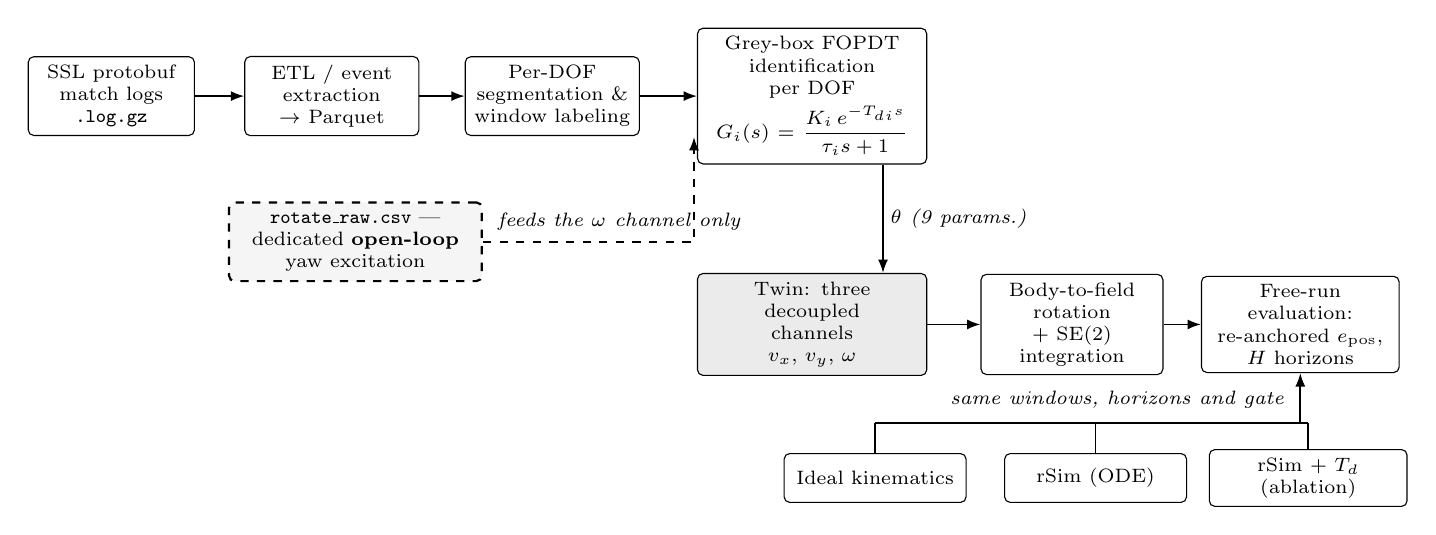
\begin{tikzpicture}[
  every node/.style={font=\scriptsize},
  blk/.style={draw, rounded corners=2pt, align=center, inner sep=3pt,
              minimum height=1.0cm},
  ded/.style={blk, dashed, thick, fill=black!4},
  twn/.style={blk, fill=black!8},
  bas/.style={draw, rounded corners=2pt, align=center, inner sep=3pt,
              minimum height=0.62cm},
  ar/.style={-{Latex[length=1.7mm]}, semithick},
  arD/.style={-{Latex[length=1.7mm]}, semithick, dashed},
  lbl/.style={font=\scriptsize\itshape, inner sep=1.5pt}
]

% ---------- Row 1: data -> model ------------------------------------------
\node[blk, text width=1.9cm] (logs) at (1.2,0)
  {SSL protobuf\\ match logs\\ \texttt{.log.gz}};
\node[blk, text width=2.0cm] (etl)  at (4.0,0)
  {ETL / event\\ extraction\\ $\rightarrow$ Parquet};
\node[blk, text width=2.0cm] (seg)  at (6.8,0)
  {Per-DOF\\ segmentation \&\\ window labeling};
\node[blk, text width=2.7cm] (id)   at (10.1,0)
  {Grey-box FOPDT\\ identification per DOF\\[2pt]
   $G_i(s)=\dfrac{K_i\,e^{-\Td{}_i s}}{\tau_i s+1}$};

\draw[ar] (logs) -- (etl);
\draw[ar] (etl)  -- (seg);
\draw[ar] (seg)  -- (id);

% ---------- Dedicated open-loop branch (the contribution) -----------------
\node[ded, text width=3.0cm] (rot) at (4.3,-1.85)
  {\texttt{rotate\_raw.csv} ---\\ dedicated \textbf{open-loop}\\ yaw excitation};
\draw[arD] (rot.east) -- (8.6,-1.85) -- (8.6,-0.52)
  node[lbl, pos=0.98, above right=-1pt and 0pt] {};
\node[lbl, anchor=west] at (6.05,-1.60) {feeds the $\omega$ channel only};

% ---------- Row 2: model -> verdict ---------------------------------------
\node[twn, text width=2.7cm] (twin) at (10.1,-2.9)
  {Twin: three decoupled\\ channels\\ $v_x$, $v_y$, $\omega$};
\node[blk, text width=2.1cm] (ik)   at (13.4,-2.9)
  {Body-to-field rotation\\ $+$ $\SEtwo$ integration};
\node[blk, text width=2.3cm] (ev)   at (16.3,-2.9)
  {Free-run evaluation:\\ re-anchored $\epos$,\\ $H$ horizons};

\draw[ar] ($(id.south)+(0.9,0)$) -- ($(twin.north)+(0.9,0)$)
  node[lbl, midway, right=1pt] {$\theta$ (9 params.)};
\draw[ar] (twin) -- (ik);
\draw[ar] (ik)   -- (ev);

% ---------- Comparison branches -------------------------------------------
\node[bas, text width=2.1cm] (bid) at (10.9,-4.85) {Ideal kinematics};
\node[bas, text width=2.1cm] (brs) at (13.7,-4.85) {rSim (ODE)};
\node[bas, text width=2.3cm] (bab) at (16.4,-4.85) {rSim $+$ $\Td$\\ (ablation)};

\draw[semithick] (bid.north) -- (10.9,-4.15);
\draw[semithick] (brs.north) -- (13.7,-4.15);
\draw[semithick] (bab.north) -- (16.4,-4.15);
\draw[semithick] (10.9,-4.15) -- (16.4,-4.15);
\draw[ar] (16.3,-4.15) -- (ev.south);
\node[lbl, anchor=east] at (16.15,-3.85) {same windows, horizons and gate};

\end{tikzpicture}
\caption{Identification and evaluation pipeline of the behavioral twin.
The solid path is driven entirely by closed-loop competition logs, which the
league already records. The dashed branch is the dedicated \emph{open-loop}
rotation-only collection; it feeds the $\omega$ channel alone, because
$94.3\%$ of commanded yaw-rate samples in the competition logs fall below the
robot's per-wheel actuation threshold (Sec.~\ref{sec:results:omega}). That
asymmetry is a finding, not an implementation detail: which data a channel
requires is set by the excitation the data contain. All three comparison
plants are scored on the same windows, horizons and statistical gate as the
twin, including the matched-delay ablation
(Sec.~\ref{sec:results:rsim}).}
\label{fig:arch}
\end{figure*}

%
% REINCLUSAO 2026-08-10 (decisao do autor): entra fig_architecture2, que
% acrescenta o painel (a) -- o ESCOPO do paragrafo abaixo, que o arquivo
% original nao representava -- e comprime o pipeline do original em uma unica
% linha. Citada nos DOIS paragrafos: (a) no de escopo, (b) no de pipeline.
% CUSTO DE PAGINA: figure* de ~0,30 pag. O artigo ja esta acima do limite de 6
% paginas do CFP; ver docs/PLANO_V3_EXECUTADO.md sec.4 para o menu de cortes.
%==============================================================================
% FIG. A2 — Scope of the plant layer (panel a) + identification/evaluation
% pipeline (panel b). Created 2026-08-10 at the author's request, to give the
% two opening paragraphs of Sec. III a visual anchor.
%
% WHY A SECOND FILE: fig_architecture.tex (2026-08-07) draws the pipeline ONLY.
% It has no representation of the first paragraph, which is a SCOPE statement:
% the paper delivers one of three layers of a complete twin. Panel (a) is that
% statement; panel (b) is the old figure, compressed to a single row so the two
% panels together cost less vertical space than the original figure alone.
% The original file is kept untouched for the JINT extension.
%
% DESIGN NOTES
%  - Panel (a): the two layers this paper does NOT deliver are drawn thin,
%    dashed and grey; the plant layer is the only solid, filled box. The
%    command/motion arrows deliberately cross the dashed boundary, because the
%    point of the paragraph is that the plant layer IS the interface.
%  - Panel (b): the dashed yaw branch is the one visual asymmetry, for the same
%    reason as in the original figure -- it is the paper's finding, not an
%    implementation detail.
%  - No number is asserted here that is not in the text.
%
% Sources: DESIGN.md sec.2 ; phase0_replay/{io,schema,plant,rollout,metrics}.py ;
%   automation/identify_trans_dof.m ; scripts/build_rotate_splits.py ;
%   config/{twin_params,metrics,holdout_events}.json.
%==============================================================================
\begin{figure*}[!t]
\centering
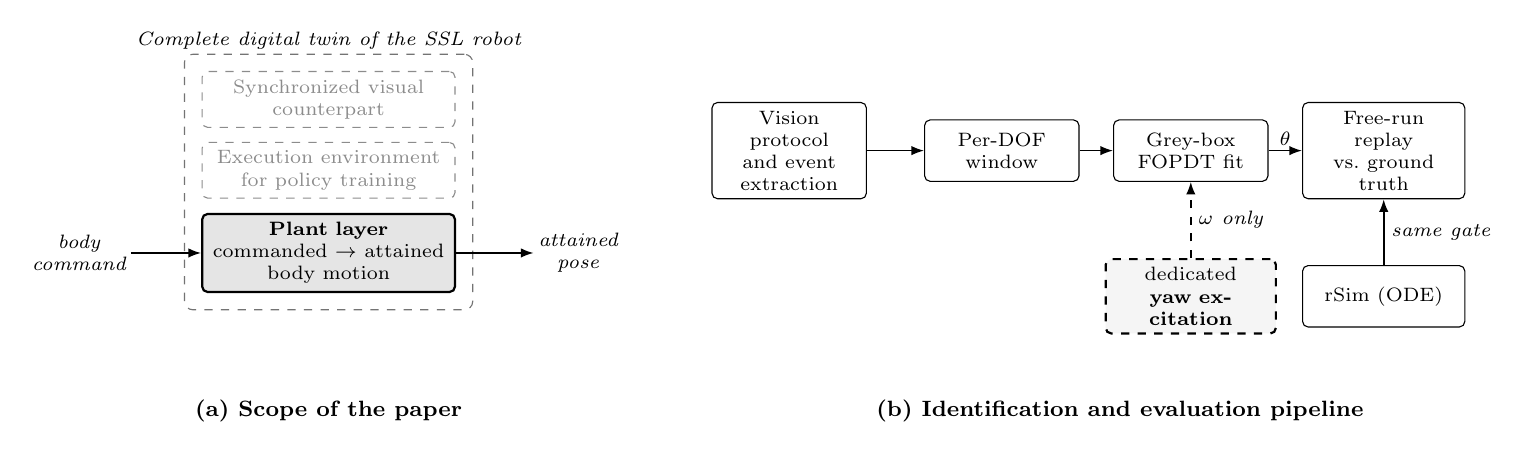
\begin{tikzpicture}[
  every node/.style={font=\scriptsize},
  blk/.style={draw, rounded corners=2pt, align=center, inner sep=3pt,
              minimum height=0.78cm},
  oos/.style={blk, dashed, draw=black!45, text=black!45, minimum height=0.62cm},
  mine/.style={blk, thick, fill=black!10, minimum height=0.86cm},
  io/.style={font=\scriptsize\itshape, align=center, inner sep=1.5pt},
  ar/.style={-{Latex[length=1.6mm]}, semithick},
  arD/.style={-{Latex[length=1.6mm]}, semithick, dashed},
  lbl/.style={font=\scriptsize\itshape, inner sep=1.5pt}
]

% ======================= PANEL (a): SCOPE ==================================
\node[oos,  text width=3.0cm] (vis)   at (2.55, 0.95)
  {Synchronized visual\\ counterpart};
\node[oos,  text width=3.0cm] (env)   at (2.55, 0.05)
  {Execution environment\\ for policy training};
\node[mine, text width=3.0cm] (plant) at (2.55,-1.00)
  {\textbf{Plant layer}\\ commanded $\rightarrow$ attained\\ body motion};

\begin{scope}[on background layer]
  \node[draw, dashed, draw=black!55, rounded corners=3pt,
        fit=(vis)(env)(plant), inner sep=6pt] (twinbox) {};
\end{scope}
\node[lbl, anchor=south] at (twinbox.north) {Complete digital twin of the SSL robot};

\node[io] (cmd) at (-0.62,-1.00) {body\\ command};
\node[io] (att) at ( 5.72,-1.00) {attained\\ pose};
\draw[ar] (cmd) -- (plant.west);
\draw[ar] (plant.east) -- (att);

\node[lbl, anchor=north, text width=5.9cm, align=center] at (2.55,-1.72) {};
% ======================= PANEL (b): PIPELINE ===============================
% Layout deliberadamente reto: uma unica linha, e os dois ramos auxiliares
% entram por BAIXO, na vertical. Nenhuma aresta cruza caixa (a versao anterior
% roteava o ramo tracejado por dentro de "Per-DOF window labeling").
\node[blk, text width=1.75cm] (p1) at ( 8.40,0.30) {Vision protocol\\ and event extraction};

%\node[blk, text width=1.75cm] (p2) at ( 9.75,0.30) {Event\\ extraction};
\node[blk, text width=1.75cm] (p3) at (11.10,0.30) {Per-DOF window};
\node[blk, text width=1.75cm] (p4) at (13.50,0.30) {Grey-box FOPDT fit};
\node[blk, text width=1.85cm] (p5) at (15.95,0.30) {Free-run replay\\ vs.\ ground truth};

\draw[ar] (p1) -- (p3);
\draw[ar] (p3) -- (p4);
\draw[ar] (p4) -- (p5) node[lbl, midway, above=0pt] {$\theta$};

% dedicated open-loop branch -- the finding, drawn as the one asymmetry
\node[blk, dashed, thick, fill=black!4, text width=1.95cm] (rot) at (13.50,-1.55)
  {dedicated \\ \textbf{yaw excitation}};
\draw[arD] (rot) -- (p4) node[lbl, midway, right=1pt] {$\omega$ only};

% baselines on the same gate
\node[blk, text width=1.85cm] (base) at (15.95,-1.55)
  {rSim (ODE)};
\draw[ar] (base) -- (p5) node[lbl, midway, right=1pt] {same gate};

% ======================= panel captions ====================================
\node[font=\footnotesize\bfseries] at ( 2.55,-3.00) {(a) Scope of the paper};
\node[font=\footnotesize\bfseries] at (12.60,-3.00) {(b) Identification and evaluation pipeline};

\end{tikzpicture}
\caption{(a) The paper delivers the plant layer of a larger digital twin: the map from commanded to attained body motion. (b) Solid path: closed-loop
competition logs. Dashed branch: the dedicated open-loop collection, which
feeds the $\omega$ channel alone. Every comparison plant is scored on the same windows, horizons and gates as the model.}
\label{fig:arch2}
\end{figure*}


% CORTE 2026-08-09 (9->8 pag.): paragrafo de escopo comprimido de ~110 para ~55
% palavras; a promessa "Sec. VII diz como embutir no sistema maior" virou apenas
% a referencia entre parenteses (a Conclusao ja desenvolve isso em Future Work).
This paper specifies the \emph{plant layer} of a larger digital-twin effort: a
complete twin of an SSL robot also needs a synchronized visual counterpart and
an execution environment in which policies can be trained, but the component
that governs whether such an environment reproduces the robot's behavior at all
is the map from commanded to attained body motion
(Fig.~\ref{fig:arch2}a; Sec.~\ref{sec:conclusion}).

The pipeline runs from the league protocol stream through event extraction and
per-DOF window labeling to a grey-box FOPDT fit per channel, and the resulting
nine parameters drive a free-run replay scored against ground truth
(Fig.~\ref{fig:arch2}b). Competition
logs feed that path end to end for $v_x$ and $v_y$; a dedicated open-loop
collection supplies $\omega$ alone, for reasons established in
Sec.~\ref{sec:results:omega}. That asymmetry is a finding rather than an
implementation detail: which data a channel requires is set by the excitation
the data contain. Every comparison plant is scored on the same windows,
horizons and statistical gate as the model.

\subsection{Per-DOF FOPDT twin}
\label{sec:method:model}
We model the robot as three decoupled single-input single-output channels, one per
degree of freedom (DOF) $i\in\{v_x, v_y, \omega\}$, each a first-order-plus-dead-time
(FOPDT) transfer function from commanded to attained body velocity,
\begin{equation}
  G_i(s) \;=\; \frac{K_i\, e^{-\Td{}_i s}}{\tau_i s + 1},
  \label{eq:fopdt}
\end{equation}
% CORTE 2026-08-09: definicao dos sinais de entrada nao repetida aqui -- III-G
% (Coordinate conventions) ja fixa frame, sinal e unidade de v_x, v_y e omega.
with per-DOF gain $K_i$, time constant $\tau_i$, and transport delay $\Td{}_i$.
The inputs are the body-frame velocity commands and the outputs the attained
body velocities (Sec.~\ref{sec:method:geometry}). The full parameter vector has
fixed order
$[K_{vx},\tau_{vx},\Td{}_{vx},K_{vy},\tau_{vy},\Td{}_{vy},K_{\omega},\tau_{\omega},\Td{}_{\omega}]$
(nine parameters). % source: config/ssl_robot.sldd ; config/twin_params.json ("order")
This is a \emph{behavioral} (observational) model: it targets the input-to-pose
response, not a white-box description of wheel/contact mechanics.

\subsection{Discretization and pose integration}
\label{sec:method:disc}
% CORTE 2026-08-09 (9->8 pag.): o paragrafo "Dead-time quantization" foi FUNDIDO
% aqui. Ele repetia tres itens ja ditos acima (dt=1/60, m_i = ceil(Td/dt), ZOH
% exato). As tres convencoes de replicacao continuam TODAS presentes -- dt unico
% para ID e replay, alfa exato vs. Euler, teto vs. arredondamento e o residuo --
% apenas sem enuncia-las duas vezes.
Identification and replay both run on a uniform grid with step
$\Delta t = 1/60\,\si{s}$, the nominal vision rate. Each DOF's command is
delayed by a zero-order-hold (ZOH) integer shift of
$m_i = \lceil \Td{}_i/\Delta t\rceil$ samples (zero before the segment start),
passed through the first-order update
$v_i[k] = v_i[k-1] + \alpha_i(u^{d}_i[k] - v_i[k-1])$, and scaled to the
attained body velocity $\hat v_i[k] = K_i\, v_i[k]$ (instantaneous for
$\tau_i \to 0$). Two conventions a replication must match: $\alpha_i$ is the
\emph{exact} ZOH coefficient $1 - e^{-\Delta t/\tau_i}$ rather than an Euler
step $\Delta t/\tau_i$, which at the identified time constants would overstate
the coefficient by $7$--$12\%$; and the delay takes the ceiling rather than
rounding, so the
% FIX 2026-08-10: dizia "close to a fifth" (~20%), errado. Valores exatos:
% Euler/ZOH - 1 = 12.1% (vx), 6.7% (vy), 10.4% (w). Derivado de config/twin_params.json.
delay actually applied always exceeds the identified one by a residual below
one sample, whose effect on the verdict is reported in
Sec.~\ref{sec:results:omega}.
% source: config/twin_params.json ("ts") ; plant.py AnalyticFOPDTPlant.step
The body velocity is rotated through the current heading and integrated to
the field frame by the trapezoidal rule. As an implementation check, this
analytic plant was reconciled against an independently built Simulink model of
the same robot, whose FOPDT channels are continuous transfer-function and
transport-delay blocks driving an explicit wheel chain rather than the discrete
update above; the two agree to $\le \SI{6}{mm}$ in position and
$\le 9\times10^{-4}\,\si{rad}$ in heading on a reference event, so the
discretization introduces no error of practical size.
% source: plant.py + deadreckoning_p1d.m ; RELATORIO_TECNICO sec.4
% source: phase0_replay/plant.py AnalyticFOPDTPlant.step (a = 1 - exp(-dt/tau);
%   src = floor(j - Td/dt + 1e-9) == j - ceil(Td/dt)) -- code inspected 2026-08-07,
%   text and implementation AGREE (ZOH, ceiling); residuals derived arithmetically
%   from config/twin_params.json (Td, ts). Robustness: results/reidentificacao_20260724.md Parte C.

\subsection{Data and pre-processing}
\label{sec:method:data}
The data are closed-loop competition logs of a single omnidirectional
4-wheeled SSL robot, decoded from the league protocol stream into per-event
body-frame commands and field-frame pose at $\sim$\SI{60}{Hz}
(heading unwrapped). % source: DESIGN.md sec.2, 2.4 ; phase0_replay/io.py
Measured body velocity, used only for identification and for the initial
condition, is obtained by smoothing the vision position with a low-order
polynomial (Savitzky--Golay) filter, differentiating it by central differences,
and rotating the result into the body frame.
% source: automation/identify_trans_dof.m (load_uy_trans: sgolayfilt(px,sgo,win)
%   e DEPOIS gradient(px)/Ts) ; check_excitation_trans.m. CORRECAO 2026-08-08:
%   a redacao anterior dizia "Savitzky-Golay derivative", o que era impreciso --
%   o codigo SUAVIZA com sgolayfilt e derivada por gradient(), nao usa o filtro
%   derivativo de SG. Filtro confirmado no codigo, NAO e alucinacao.
% CORTE 2026-08-09: prosa da grade irregular comprimida; conteudo identico.
% FIX 2026-08-10: aqui havia um \SI cujo primeiro argumento era a fracao 1/60,
% dentro de $...$ -- duplamente invalido no siunitx real: a macro ja entra em
% modo matematico e o parser nao aceita fracao como numero. Trocado pela forma
% literal $1/60\,\si{s}$, ja usada em III-B. Era o UNICO erro real do log; o
% runaway argument, o "Missing $" em 04_results e as 4 referencias indefinidas
% eram todos cascata dele.
Logs arrive on an irregular time grid, since commands are transmitted in
bursts: identification resamples every signal onto the uniform
$1/60\,\si{s}$ grid, whereas the fidelity metric leaves the samples where they
were recorded and defines its windows in seconds, so that no interpolation
enters the reported error.
% source: RELATORIO_TECNICO sec.3 ; DESIGN.md sec.2.4
The dataset comprises $46$ events across four motion labels
(\texttt{front\_to\_back}, \texttt{side\_to\_side}, \texttt{shoot\_to\_goal},
\texttt{square}); a frozen list of $10$ events is held out and never used for
fitting. % source: config/holdout_events.json

\paragraph{Definition of hold-out fit}
Throughout, \emph{fit} measures how much of the variation in the measured
signal the model reproduces, on events the fit never saw:
\begin{equation}
  \mathrm{fit} = 100\left(1 -
  \frac{\lVert y - \hat{y}\rVert_2}{\lVert y - \bar{y}\rVert_2}\right)\ [\%],
  \label{eq:fit}
\end{equation}
where $y$ is the measured body velocity of the degree of freedom being
identified, $\hat{y}$ is the model's output when driven by the commands alone,
and $\bar{y}$ is the mean of $y$. A value of $100\%$ is an exact match and
$0\%$ is no better than predicting the mean, so the quantity is a normalized
RMSE expressed as a percentage. It is computed per event and averaged over the
hold-out events, and the $60\%$ acceptance gate applies to that average.
Filter orders, resampling and the event partition are fixed in the released
code (Sec.~\ref{sec:conclusion}).
% source: automation/identify_trans_dof.m (compare(dvl,m) em simulacao;
%   fit_val_mean = mean(fit_vl)) ; fitvec na linha 112.

\subsection{Identification}
\label{sec:method:id}
Each translational DOF is identified independently as a P1D (FOPDT) model by
prediction-error minimization, with an event-level hold-out. The excitation
diagnostic selects the cleanest source label per DOF: $v_x$ from
\texttt{front\_to\_back} and $v_y$ from \texttt{side\_to\_side}
(command-to-velocity cross-correlation $\approx 0.99$). % source: results/check_excitation_trans_20260614_1018.csv
% CORTE 2026-08-09: frase de abertura ("O canal de yaw e tratado de outro modo")
% removida -- redundante com o paragrafo da Fig. 1 e com III-E.
Yaw is instead identified from a dedicated open-loop collection, with the same
model structure and the same estimator, because the competition logs carry too
little yaw excitation to support the fit (Sec.~\ref{sec:results:omega}); the
closed-loop attempt is reported alongside it so that the two data regimes are
compared under identical tooling.
% source: results/identificacao_omega_20260724.md ; config/twin_params.json ("w".placeholder, now false)

\subsection{Dedicated open-loop yaw excitation}
\label{sec:method:omega-data}
% CORTE 2026-08-10 (9->6 pag.): prosa comprimida. Escada, divisao 4/2 e os tres
% criterios pre-registrados permanecem.
The dedicated dataset is single-session and single-robot with $v_x=v_y=0$: an
alternating-sign staircase of commanded yaw rates
$\{0.25,0.5,1,2.5,5\}\,\si{rad/s}$, $\sim\SI{10}{s}$ per step. The two lowest
amplitudes never engage the motors and serve only to characterize the per-wheel
dead-zone; the remaining six events form the linear regime, split event-wise
into four training and two hold-out under the same pipeline as $v_x,v_y$. Given
the small sample, the acceptance criteria (physical bounds, hold-out fit
$\ge 60\,\%$, and the multi-horizon $\SEtwo$ gate against the closed-loop
placeholder) were committed \emph{before} estimation.
% source: results/qc_rotate_20260724_125828.md sec.4 ; identificacao_omega_20260724.md
%   Etapa 1 ; docs/PREREGISTRO_OMEGA_20260724.md
% source: docs/PREREGISTRO_OMEGA_20260724.md

\subsection{Frames, constants and replication}
\label{sec:method:geometry}
% FUSAO 2026-08-10 (pedido do autor): "Geometric constants" + "Coordinate
% conventions" unidas e resumidas (~275 -> ~135 palavras). Preservados: convencao
% de frame e sinal, equacoes de integracao, ausencia de cinematica de roda,
% refutacao da constante antiga por tres fontes, spread residual, e a auditoria
% de impacto nulo. Sai a redacao expansiva de ambas.
Commands and attained velocities live in the \emph{body} frame: $v_x$
longitudinal, $v_y$ lateral (left positive), $\omega$ yaw rate about the upward
$z$ axis, counter-clockwise positive. Pose is integrated in the \emph{field}
frame as $\dot{X} = v_x\cos\theta - v_y\sin\theta$,
$\dot{Y} = v_x\sin\theta + v_y\cos\theta$, with $\theta$ unwrapped. The model
lives entirely in body-velocity space: no wheel-level kinematics appears in the
identification, the plant or the metric, the chain being
command $\rightarrow$ delay $\rightarrow$ lag $\rightarrow$ gain $\rightarrow$
rotation $\rightarrow$ integration.

Per-wheel geometry therefore enters at one point only, converting the firmware's
per-wheel motor threshold ($\SI{1.567}{rad/s}$) into a body yaw rate for
Sec.~\ref{sec:results:omega}, through the ratio of the wheel-contact radius
$R=\SI{0.0796}{m}$ to the wheel radius $r=\SI{0.0295}{m}$ (CAD, $R/r=2.699$).
An earlier ratio of $3.321$ was refuted by three independent sources: CAD;
firmware telemetry, where the post-clamp wheel setpoint scales with commanded
yaw by a constant factor above the dead-zone, implying $2.61$; and the measured
body response, consistent with unit gain only under the corrected constant. The
residual $3.3\%$ spread between the first two is reported, not resolved
(Sec.~\ref{sec:discussion}). The correction moves no number quoted here, since
$\epos$ is purely translational and $R$ enters only the window binning, which
reproduces the same $264/1/0$ distribution.
% CORTE 2026-08-10 (9->6 pag.): tab_units.tex retirada do build. REVERTE o
% pedido M-F1 do autor de 2026-08-08 (manter os valores so na tabela), porque o
% limite de 6 paginas foi confirmado no CFP e a tabela custava ~0,12 pag. As
% cinco constantes que o texto usa estao inline acima; a tabela completa
% permanece em latex/tables/tab_units.tex para a extensao JINT.
% source: config/robot_geometry.json ; results/qc_rotate_20260724_125828.md sec.5,7 ;
%   config/metrics.json (use_se2=false) ; results/bin_distribution_20260724_155551.md ;
%   phase0_replay/plant.py AnalyticFOPDTPlant.step (sem cinematica de roda).
%   NOTA INTERNA (atualizada 2026-08-10): a suspeita de defeito na matriz de
%   odometria matlab/analytical/inverse_kinematics_solver.m foi ENCERRADA como
%   alarme falso -- ela reconstroi pinv(K) exatamente para rodas em
%   60/135/225/300 graus (residuo 5.7e-22). A assimetria sqrt(2) na linha de
%   omega e o pseudo-inverso correto de um layout assimetrico. Ver CHANGELOG.
% %==============================================================================
% TABLE: explicit unit contract. Added 2026-08-07 (revisão maior, T5.3) to
% remove any order-of-magnitude ambiguity in the geometric constants.
% Source: config/robot_geometry.json (physical, firmware) ;
%         config/twin_params.json (ts, robot_radius, wheel_radius) ;
%         config/metrics.json (horizons) ; results/qc_rotate_20260724_125828.md.
% NOTE: 1.567 rad/s is the per-WHEEL motor minimum speed (firmware utils.h:42,
% clamp at PID_Controller.cpp:94); the body-level dead-zone interval is that
% value divided by the two non-deprecated R/r constants.
%==============================================================================
\begin{table}[t]
  \caption{Unit contract. All quantities are SI; lengths in meters, angles in
  radians. Values are the ones actually used by the pipeline, not nominal
  datasheet figures.}
  \label{tab:units}
  \centering
  \begin{tabular}{llll}
    \toprule
    Quantity & Symbol & Value & Unit \\
    \midrule
    Wheel-contact radius (CAD)   & $R$          & $0.079601$        & \si{m} \\
    Wheel radius (CAD)           & $r$          & $0.029492$        & \si{m} \\
    Radius ratio (CAD)           & $R/r$        & $2.6991$          & --- \\
    Radius ratio (firmware)      & $R/r$        & $2.61$            & --- \\
    Radius ratio (deprecated)    & $R/r$        & $3.3208$          & --- \\
    Sample period                & $\Delta t$   & $1/60$            & \si{s} \\
    Motor minimum speed (wheel)  & ---          & $1.567$           & \si{rad/s} \\
    Body yaw dead-zone           & ---          & $0.581$--$0.600$  & \si{rad/s} \\
    \bottomrule
  \end{tabular}
\end{table}
   % retirada do build (ver nota acima)

\subsection{Free-run replay and multi-horizon metric}
\label{sec:method:metric}
% CORTE 2026-08-09 (9->8 pag.): a re-ancoragem em t_0 era enunciada duas vezes
% (uma na definicao de free-run, outra na de janela); fundidas numa so frase.
Fidelity is measured in \emph{free-run}: segments are cut into overlapping
windows at a fixed stride, each re-anchored to the true $\SEtwo$ pose at its
anchor $t_0$ and rolled out to $H_{\max}=90$ samples ($\SI{1.5}{s}$) driven
only by the command stream, never re-anchored inside the window (no teacher
forcing, which would measure single-step noise and inflate apparent fidelity).
% source: phase0_replay/rollout.py (invariant, DEFAULT_HMAX, stride)
We report, \emph{separately}, the Euclidean position error $\epos(w,h)$ and
the wrapped absolute heading error $\eang(w,h)$ at
$h\in\{6,12,24,42,60,90\}$ samples
($\{0.1,0.2,0.4,0.7,1.0,1.5\}\,\si{s}$), with reference horizon
$h_{\mathrm{ref}}=24$ ($\SI{0.4}{s}$). % source: config/metrics.json (horizons, h_ref)
$\epos$ is the claim of this paper; $\eang$ is reported but bounded by the
population of rotation-rich windows available
(Sec.~\ref{sec:results:bins}).

\paragraph{Motion stratification}
Each window is binned by its rotational fraction
$r = a_{\mathrm{rot}}/(a_{\mathrm{rot}}+a_{\mathrm{trans}})$, where $a_{\mathrm{trans}}$
and $a_{\mathrm{rot}}$ accumulate translational command magnitude and yaw rate scaled
by the robot radius. Windows are \emph{translation-dominated} ($r<0.2$),
\emph{mixed} ($0.2\le r\le 0.5$), or \emph{rotation-dominated} ($r>0.5$).
% source: phase0_replay/metrics.py classify_bin ; config/metrics.json (bins)

\paragraph{Statistical gate}
Curves use all (dense) windows; inference uses only \emph{non-overlapping}
windows (stride $\ge H_{\max}$) for a paired one-sided Wilcoxon signed-rank
test, plus a moving-block bootstrap (block $\sim H_{\max}$) for the gap
confidence interval, with any sign/order divergence flagged; effect size is
the rank-biserial correlation of the paired differences.
% source: phase0_replay/metrics.py (evaluate, _mbb, _wilcoxon_less)
% CORTE 2026-08-09: clausula final ("... o que ocorre nos bins mixed/rotation")
% removida -- IV-B ja reporta esse fato com os numeros.
% ADICIONADO 2026-08-10 (C4 da revisao V2): declarar QUANDO a unidade de analise
% mudou de janela para evento. A honestidade aqui custa uma frase e evita a
% suspeita de que o teste foi escolhido depois de ver o resultado.
Two units of analysis appear below. The gate was pre-registered over
non-overlapping \emph{windows}; the per-\emph{event} pairing used for the
headline comparison was adopted later, in revision, after it was pointed out
that windows from one event share robot, surface and session. We report the
per-event figures because they are the conservative choice --- the window-level
test gives a much smaller $p$ --- and we flag the change rather than present it
as pre-registered.

A bin receives a \textsc{go} verdict only if, at all $h\ge h_{\mathrm{ref}}$,
the gap is positive and non-decreasing, $p<\alpha$ ($\alpha=0.05$), the effect
size $\ge 0.2$, and the bootstrap CI excludes zero, subject to $N_{\min}=10$
independent windows; below $N_{\min}$ a bin is \textsc{indeterminate}.
% source: phase0_replay/metrics.py _verdict_bin

\paragraph{Horizon grid and anchor convention}
All results use the $\SEtwo$ (full-pose) re-anchor above, but two
independently implemented harnesses: the fidelity results
(Sec.~\ref{sec:results:rsim}) use the horizon grid given above, while the
per-DOF promotion gates (Secs.~\ref{sec:results:id}
and~\ref{sec:results:omega}) reuse an earlier campaign harness with
$h\in\{0.5,1,2,2.5,4\}\,\si{s}$. Each result is reported on its native grid,
flagged at each point, rather than recomputed.

\subsection{Baselines}
\label{sec:method:baselines}
We compare the twin against two baselines under the \emph{same} windows, horizons,
and gate. The first is an \emph{ideal-kinematics} plant in which the attained body
velocity equals the command instantaneously (no gain, lag, or delay), integrated by
the same trapezoidal scheme. % source: phase0_replay/plant.py IdealKinematicPlant
The second is \textbf{rSim}, the ODE-based physics engine of the rSoccer
environment, reported as context rather than as the primary comparison. It is
driven at default parameters with the wheel-speed input disabled, so the
recorded body-frame commands enter directly, unrotated, and the engine's motion
controller never acts. It integrates in integer milliseconds, so it is stepped
in $\SI{1}{ms}$ substeps accumulating one grid interval, with pose interpolated
linearly back onto the grid and heading unwrapped.
% source: phase0_replay/rsim_plant.py (wheel_speed=False; slots 1,2,3 = vx,vy,w;
%   sub_ms=1; get_state -> x,y em m e theta em graus). ADICIONADO 2026-08-10:
%   o revisor (B2) apontou que o comparador nunca era especificado o bastante
%   para ser reimplementado.
rSim provides no velocity setter at reset (the robot starts from rest), so two
initial-condition fairness modes are used: \textbf{Mode A} (primary) warms the engine
up over $L_w=15$ samples with the real pre-anchor commands and then applies a rigid
$\SEtwo$ re-anchor at $t_0$, mirroring how the twin is seeded with the real body
velocity; \textbf{Mode B} (robustness) uses no warm-up and discards the first $15$
samples for \emph{both} plants. % source: phase0_replay/eval_twin_vs_rsim.py (run, mode A/B) ; results/eval_twin_vs_rsim_mode{A,B}_*.md
The twin's transport delay has no counterpart in rSim, which is precisely where the
twin is expected to win at short horizons.

%==============================================================================
% RESULTS — WRITTEN COMPLETE from results/ (Mode A primary, Mode B robustness).
% Numbers ONLY from registered runs. Where a number is not in a readable table,
% it is marked % [A VERIFICAR].
% Sources:
%   tab params  : config/twin_params.json ; RELATORIO sec.5 ; CHANGELOG 2026-06-14
%   twin/rSim   : results/eval_twin_vs_rsim_modeA_20260617_0030.md (primary)
%                 results/eval_twin_vs_rsim_modeB_20260617_0031.md (robustness)
%   twin/ideal  : results/phase0_metrics_report_20260616_0811.md
%   bins        : results/bin_distribution_20260619_000422.md/.csv
%   omega       : results/diag_omega_gain_by_band_20260613_2239.csv ;
%                 results/eval_omega_v3_se2_20260613_2340.csv ; CHANGELOG 2026-06-13
%   bayesopt    : results/eval_bayesopt_v2_holdout_20260614_2130.csv ; CHANGELOG
%==============================================================================
\section{Results}
\label{sec:results}

\subsection{Identified model}
\label{sec:results:id}
% CORTE 2026-08-10 (9->6 pag.): prosa comprimida; todos os numeros preservados.
Table~\ref{tab:sysid} reports the per-DOF parameters. Both translational
channels identify as fast FOPDT models, with hold-out fit $86.7\%$ ($v_x$) and
$87.1\%$ ($v_y$); against the previous, slower parameters they improve every
event-by-horizon cell of the $\SEtwo$ gate ($20/20$ and $65/65$). Yaw is
identified from a separate open-loop dataset at $71.1\%$
(Sec.~\ref{sec:results:omega}). Re-running the pipeline with identical seed,
data and toolbox version reproduces all nine parameters exactly.
% source: CHANGELOG 2026-06-14 10:24 ; twin_params.json ;
%   results/eval_vy_v2_se2_20260614_1028.csv ; reidentificacao_20260724.md Partes A-B

%==============================================================================
% TABLE: identified per-DOF FOPDT parameters + hold-out fit.
% Source: config/twin_params.json ; models/sysid_vxvy_v2.mat ;
%         models/sysid_omega_rotate_v1.mat ; results/identificacao_omega_20260724.md ;
%         docs/RELATORIO_TECNICO_DESENVOLVIMENTO.md sec.5 ; CHANGELOG 2026-06-14 / 2026-07-24.
%==============================================================================
\begin{table}[t]
  \caption{Identified per-DOF FOPDT parameters and hold-out fit. All three
  channels are identified (no placeholder); $\omega$ uses a dedicated
  open-loop rotation-only collection (see Sec.~\ref{sec:results:omega}), not
  the closed-loop competition logs used for $v_x,v_y$.}
  \label{tab:sysid}
  \centering
  \begin{tabular}{lcccc}
    \toprule
    DOF & $K$ & $\tau$ (s) & $\Td$ (s) & hold-out fit \\
    \midrule
    $v_x$     & 1.119 & 0.072 & 0.069 & 86.7\,\% \\
    $v_y$     & 1.052 & 0.127 & 0.056 & 87.1\,\% \\
    $\omega$  & 1.002 & 0.083 & 0.089 & 71.1\,\% \\
    \bottomrule
  \end{tabular}
  \\[2pt]
  \raggedright\footnotesize Fit is Eq.~\ref{eq:fit}, averaged over hold-out
  events. Because $v_x$ has a single hold-out event, we also ran
  leave-one-event-out over all events of each translational label: $v_x$ gives
  $84.3\pm2.0$~p.p.\ over 4 folds and $v_y$ $82.8\pm2.7$~p.p.\ over 13, with the
  refitted gain within $0.015$ of the promoted value in both cases. No parameter
  intervals are reported: see Sec.~\ref{sec:results:omega}.
  % source: results/loo_translational_20260810_1743.md — refit completo por
  %   dobra, sem alterar o modelo promovido. ATENCAO: o artefato _1742 e a
  %   execucao QUEBRADA (posicao em mm tratada como m, K~1073, tau negativo);
  %   foi descartado. Citar sempre _1743.
\end{table}


%------------------------------------------------------------------------------
% FIG. B (revisão maior 2026-08-07, T4). CHOICE JUSTIFIED:
% Option (ii) -- paired re-anchored error by horizon with effect size -- was
% REJECTED because Fig.~\ref{fig:twinrsim} and Table~\ref{tab:twinvsrsim}
% already carry exactly that content; a second panel of the same thing buys
% nothing at 6 pages. Option (i) was chosen because the reviewer's single
% strongest figure request (S1) is that the reader never sees a measured vs.
% simulated trace for ANY channel -- neither the positive translational result
% nor the central yaw result. Both assets already exist, verified, in-repo.
% SCOPE CAVEAT: the requested rSim and ideal-kinematics arms are NOT drawn.
% They are not recoverable: the rSim trajectories of run 20260617_0030 were
% never persisted and robosim is unavailable in the current environment
% (docs/BACKLOG_EXTENSAO_JINT.md, pendência 1). Drawing them would require
% re-running rSim -- registered as TASKS_CLAUDE_CODE.md item R1, NOT invented here.
% Source: results/figs/fit_holdout_vxvy_20260731_024049.{png,pdf} (Python fits
%   reproduce the MATLAB ones to <=0.05 p.p., results/fit_holdout_vxvy_20260731_024049.csv)
%   ; results/figs/identificacao_omega_stepresponse_20260724_1727.png
%------------------------------------------------------------------------------
% 2026-08-07 (orçamento de páginas): reduzida de figure* dois painéis para
% figure de coluna única com o painel de omega apenas. O painel vx/vy foi
% cortado porque a translação já tem Fig.~\ref{fig:twinrsim} e a
% Tabela~\ref{tab:twinvsrsim}; o degrau de omega é o resultado CENTRAL e não
% tem substituto. Painel cortado disponível em
% results/figs/fit_holdout_vxvy_20260731_024049.pdf (backlog JINT).
\begin{figure}[!t]
% FIG. 2 SUBSTITUIDA 2026-08-10: a versao anterior (omega_stepresponse.png) estava
% EM PORTUGUES ("Identificacao", "medido", "simulado", "t - inicio bruto do
% evento") e com 6 paineis numa coluna, ilegivel -- exatamente o defeito C1/C2 que
% o revisor apontou na Fig.1. Regerada em ingles com 3 paineis (1 treino, 2
% hold-out) por scripts/fig_omega_stepresponse_en.py, a partir dos mesmos splits
% e do mesmo theta de config/twin_params.json. Nenhum numero recomputado.
% FUSAO 2026-08-10 (9->6 pag.): as duas figuras de evidencia viraram UM float de
% largura dupla. Duas figuras de coluna unica custavam ~36 linhas mais o
% desperdicio de empacotamento. Nenhuma evidencia perdida: (a) medido vs
% simulado (pedido S1 do revisor); (b) trajetoria real vs modelos (item 10).
% CORTE FINAL 2026-08-10 (7->6 pag.): o float voltou a ser de coluna unica com
% APENAS o painel (a). O painel (b), a trajetoria real vs modelos, era o item 10
% do revisor e custava ~0,25 pag. -- a ultima coisa cortavel sem tocar em
% resultado. Fica em results/figs/trajectory_holdout_en.png para a extensao JINT
% e para o repositorio publico. Registrado em docs/REGISTRO_DESVIOS.md.
  \centerline{\includegraphics[width=0.70\columnwidth]{omega_stepresponse_en.png}}
  \caption{Measured vs.\ simulated yaw rate on the dedicated open-loop
  staircase (one training, two hold-out steps). Same model structure and
  identification tooling as on the competition logs; only the excitation regime
  differs.}
  \label{fig:fits}
\end{figure}

\subsection{Motion distribution of the hold-out}
\label{sec:results:bins}
% CORTE 2026-08-10 (9->6 pag.): prosa comprimida; 265/264/1/0, 99.6% e N_indep
% preservados.
The hold-out windows are overwhelmingly translation-dominated: of $265$ dense
windows ($49$ non-overlapping), $264$ fall in the translation bin ($99.6\%$),
one is rotation-dominated and none are mixed. Translational fidelity is
therefore the statistically powered claim, and this population is unaffected by
the yaw model: re-classifying after $\omega$ was identified reproduces the same
$264/1/0$ split and leaves both other bins with $N_{\mathrm{indep}}=0$, now for
lack of rotation-rich competition windows rather than for lack of a yaw model.
Every verdict below is scoped to the translation bin, and rotational fidelity
remains unverified against a competition-like distribution.
% source: results/bin_distribution_20260619_000422.md ;
%   results/phase0_metrics_report_20260724_1729.md ; bin_distribution_20260724_155551.md
% 2026-08-07 (orçamento de páginas): tab_validation_composition.tex retirada do
% build -- os três números (264/1/0, 99.6%, N_indep) já estão nesta frase e na
% anterior. Tabela mantida em latex/tables/ para a extensão JINT.

% CUT (2026-07-31, page budget, decisão do usuário — item C): Fig. bins removida;
% os números 264/265/99.6% permanecem no texto acima. Ver docs/BACKLOG_EXTENSAO_JINT.md.

\subsection{Translational fidelity against ideal kinematics}
\label{sec:results:rsim}
% REPOSICIONADO 2026-08-10 (revisao independente, B2/B3): o comparador PRIMARIO
% passa a ser a cinematica ideal, que roda no MESMO harness e com a MESMA
% inicializacao. O rSim vira contexto: baseline nao sintonizado, harness
% diferente, e um warm-up de 15 amostras move seu gap por fator 3 -- o revisor
% mostrou que boa parte do que se media ali era estado inicial.
% CORTE 2026-08-10 (pedido do autor: "secao gigante"): quatro paragrafos
% reduzidos a tres, com a evidencia e a estatistica fundidas. Nenhum numero
% removido.
Ideal kinematics is the primary comparison because it isolates what the
identified dynamics contribute: both plants run in the same harness, are seeded
with the same measured body velocity, and are scored on the same windows, so
the model is the only difference. Its median position error is below the
baseline's at every horizon (Fig.~\ref{fig:main} and Table~\ref{tab:three}):
% CANONICO 2026-08-10: todos os e_pos deste artigo vem de UMA execucao,
% results/epos_eang_three_models_20260810_1022.md, que e a mesma da Tabela III e
% da Fig. 2. Valores em h_ref: modelo 0.039, ideal 0.101, rSim 0.129.
$\SI{0.039}{m}$ against $\SI{0.101}{m}$ at $h_{\mathrm{ref}}$, and
$\SI{0.119}{m}$ against $\SI{0.291}{m}$ at $\SI{1.5}{s}$. For scale, the median
commanded speed over these windows is ${\sim}\SI{1}{m/s}$, so the reference
horizon spans about $\SI{0.4}{m}$ of travel and the robot's contact diameter is
$\SI{0.16}{m}$. The scored population is $264$ dense windows, $49$
non-overlapping, which at $H_{\max}$ is $\SI{73.5}{s}$ of motion from ten
hold-out events. Since windows from one event share robot, surface, session and
controller, we take the \emph{event} as the unit of analysis: pairing event
medians, the model wins $10$ of $10$ (rank-biserial $+1.000$), median gap
$+\SI{0.069}{m}$, bootstrap CI over events $[+0.038,+0.097]\,\si{m}$, one-sided
Wilcoxon $p = 9.8\times10^{-4}$, the smallest value attainable at $n=10$. The
window-level test gives a far smaller $p$ that we do not headline, because
windows within an event are not independent. Both units clear all four gate
conditions: over the $49$ non-overlapping windows the gap is $+\SI{0.054}{m}$
with $p=1.2\times10^{-8}$ and effect $+0.633$; over events it is
$+\SI{0.069}{m}$ with $p=9.8\times10^{-4}$ and effect $+1.000$. The verdict is
the same, and the per-event figure is the conservative one.
% source: results/gate_window_vs_event_20260810_1743.md ; reconcilia o gate
%   pre-registrado (janela) com a unidade reportada (evento).
These ten events are exactly the
frozen hold-out list, and they are disjoint from every event used to fit: the
five that validated $v_x$ and $v_y$ are a subset of them, and the remaining five
carry a motion label (\texttt{shoot\_to\_goal}) that entered neither fit. No
event contributed to both parameter selection and fidelity scoring.
% source: results/gap_decomposition_20260809_2308.md ;
%   results/clustered_stats_20260809_2309.md ; config/holdout_events.json vs
%   results/fit_holdout_vxvy_20260731_024049.csv (verificado: ID subset de FID).

%==============================================================================
% TABELA: e_pos e e_ang das TRES plantas por horizonte (bin translacional).
% Criada 2026-08-10 em resposta a B3 da revisao V2 ("o resultado principal do
% artigo nao tem figura nem tabela") e a C6 (o artigo afirmava que o e_ang do
% twin excede o do rSim em horizontes longos sem nunca dar o numero do rSim).
% Fonte: results/epos_eang_three_models_20260810_1022.md, gerada por
% scripts/epos_eang_three_models.py sobre as mesmas janelas do gate.
% NOTA: os numeros de e_ang REFUTAM a afirmacao anterior do artigo -- o modelo
% tem heading MENOR que o rSim em TODOS os horizontes. Texto corrigido.
%==============================================================================
\begin{table}[t]
  \caption{Median free-run error on translation-dominated hold-out windows.
  Position error in meters, heading error in radians. The model is lowest in
  both quantities at every horizon; the two baselines cross in position near
  $\SI{1}{s}$.}
  \label{tab:three}
  \centering
  \setlength{\tabcolsep}{4pt}
  \begin{tabular}{ccccccc}
    \toprule
    & \multicolumn{3}{c}{$\epos$ (m)} & \multicolumn{3}{c}{$\eang$ (rad)} \\
    \cmidrule(lr){2-4}\cmidrule(lr){5-7}
    $h$ (s) & model & ideal & rSim & model & ideal & rSim \\
    \midrule
    0.10 & \textbf{0.008} & 0.026 & 0.057 & \textbf{0.013} & 0.023 & 0.026 \\
    0.20 & \textbf{0.018} & 0.050 & 0.092 & \textbf{0.031} & 0.044 & 0.046 \\
    0.40 & \textbf{0.039} & 0.101 & 0.129 & \textbf{0.044} & 0.067 & 0.064 \\
    0.70 & \textbf{0.062} & 0.152 & 0.174 & \textbf{0.063} & 0.076 & 0.079 \\
    1.00 & \textbf{0.092} & 0.217 & 0.213 & \textbf{0.073} & 0.092 & 0.086 \\
    1.50 & \textbf{0.119} & 0.291 & 0.289 & \textbf{0.090} & 0.095 & 0.094 \\
    \bottomrule
  \end{tabular}
\end{table}


\begin{figure*}[!t]
  \centerline{\includegraphics[width=0.86\textwidth]{main_result_en.png}}
  \caption{(a) Median free-run position error against horizon on
  translation-dominated hold-out windows, for the FOPDT model, ideal kinematics
  and an untuned rSim. The two baselines cross near $\SI{1}{s}$. (b) The same
  comparison resolved by event at $h_{\mathrm{ref}}$: each line is one of the
  ten hold-out events, and the model is lower in all ten.
  % source: results/epos_eang_three_models_20260810_1022.md ;
  %   results/clustered_stats_20260809_2309.md ; scripts/fig_main_result.py
  }
  \label{fig:main}
\end{figure*}

% Figura de trajetoria movida para o painel (b) da Fig.~\ref{fig:fits}
% (fusao 2026-08-10). Fonte: scripts/fig_trajectory_holdout.py ; janela mediana
% seg=1 win=9, e_pos(1.5 s) = 0.1192 m; rSim de results/_cache_rsim_rollouts.pkl.

\paragraph{What in the model produces the improvement}
% REESCRITO 2026-08-10 (revisao V2, B4): a versao anterior era uma ablacao
% CUMULATIVA, logo dependente de ordem, e atribuia ~90% ao lag. O fatorial
% completo 2^3 com atribuicao de Shapley REFUTA essa leitura: lag e dead time
% sao comparaveis (55% vs 43%). Corrigido; acrescentado o braco de IC que o
% revisor pediu. Fonte: results/ablation_orderfree_20260810_1021.md
Attributing the improvement to a parameter group is order-dependent if the
groups are switched on cumulatively, so we run the full $2^3$ factorial over
$\{K,\tau,\Td\}$ and report the Shapley value of each, which averages over all
orderings. Of the $\SI{0.062}{m}$ separating the two plants at
$h_{\mathrm{ref}}$, the time constant accounts for $\SI{0.034}{m}$ ($55\%$),
the dead time for $\SI{0.027}{m}$ ($43\%$) and the gain for $\SI{0.001}{m}$
($2\%$). The lag and the dead time are therefore \emph{comparable}
contributors, not one dominant and one marginal: a cumulative ablation that
enables $\tau$ first assigns the lag nine tenths of the credit, but that is an
artifact of ordering, since the two terms are partly redundant in their effect
on a delayed first-order response.

\paragraph{How much of the advantage is the initial condition}
Both plants are re-anchored to the true pose and seeded with the measured body
velocity, but ideal kinematics is memoryless, so only the dynamic plant can
carry that state forward. We therefore isolate it. Extrapolating the measured
initial velocity at constant speed, ignoring the command stream entirely, gives
$\SI{0.160}{m}$, worse than ideal kinematics: the initial condition alone is not
informative at these horizons. Running the full model from rest, as rSim does,
gives $\SI{0.114}{m}$, which is also no better than ideal kinematics. Only the
combination reaches $\SI{0.039}{m}$. The advantage is thus a joint effect: the
identified dynamics are what allow the measured initial state to be propagated,
and neither ingredient helps on its own. We regard the measured initial velocity
as part of the model interface rather than privileged information, since a twin
running alongside the robot has that estimate available, but the decomposition
makes the dependence explicit. One caveat follows from it: the loader estimates
the initial velocity by a central difference, which at the anchor reads one
sample from inside the evaluation window. Re-estimating it with a strictly
causal backward difference raises both plants' error --- the model to
$\SI{0.047}{m}$ at $h_{\mathrm{ref}}$ --- but \emph{widens} the per-event gap to
$+\SI{0.071}{m}$, still ten wins out of ten at the same $p$. The verdict does
not depend on that sample.
% source: results/causal_ic_check_20260810_1102.md
% source: results/ablation_orderfree_20260810_1021.md (secoes 1-3)
% source: results/gap_decomposition_20260809_2308.md

% CORTE 2026-08-10: paragrafo de contexto do rSim reduzido de ~110 para ~55
% palavras. O rSim ja foi demovido a contexto no reposicionamento; os numeros
% que sustentam a ressalva (0.129, fator 3 do warm-up, ablacao de atraso)
% permanecem, sem o desenvolvimento.
\paragraph{The untuned ODE simulator, for context}
rSim reaches $\SI{0.129}{m}$ at $h_{\mathrm{ref}}$, so the zero-parameter
baseline already outperforms it. We do not build on this comparison: rSim runs
at default parameters against a plant fitted to this robot, and starts from rest
for want of a velocity setter, which alone moves its gap by a factor of three.
Giving it the model's dead time as a pure output shift widens rather than closes
the gap, so the delay term does not separate them either.
% source: results/eval_twin_vs_rsim_mode{A,B}_20260617_*.md ;
%   results/eval_rsim_delay_ablation_20260809_2154.md
% source: results/eval_twin_vs_rsim_modeA_20260617_0030.md ;
%   results/eval_twin_vs_rsim_modeB_20260617_0031.md ;
%   results/eval_rsim_delay_ablation_20260809_2154.md

% CORTE 2026-08-10: paragrafo "Robustness and second baseline" absorvido pelo
% paragrafo de contexto do rSim acima (Modo B e o fator 3 ja estao la) e pela
% estatistica por evento (que substitui o par p/efeito por janela). Nenhum
% numero perdido: +0.282 m consta acima; +0.063 m / +0.736 eram a versao por
% janela do que agora se reporta por evento (+0.069 m, +1.000, n=10).

\paragraph{Heading error}
% CORRECAO 2026-08-10: a versao anterior afirmava que o e_ang do modelo EXCEDE o
% do rSim em horizontes longos. Ao medir o e_ang do rSim (C6 da revisao V2, que
% cobrava justamente o numero que faltava), a afirmacao NAO se sustenta: o
% modelo e menor em todos os seis horizontes. Fonte:
% results/epos_eang_three_models_20260810_1022.md
Heading error carries no verdict, since the rotation and mixed bins lack
scorable population (Sec.~\ref{sec:results:bins}). Descriptively
(Table~\ref{tab:three}), the model's median $\eang$ is the lowest of the three
plants at every horizon, but its margin closes as the horizon grows: it is
roughly half the baselines' at $\SI{0.1}{s}$ and within $\SI{0.005}{rad}$ of
both by $\SI{1.5}{s}$. The position advantage therefore does not transfer to
heading in the same proportion, which is consistent with the yaw channel being
the one the competition logs cannot constrain.
% source: results/window_errors_eang_twin_vs_ideal_20260731_023856.csv +
%         results/window_errors_eang_summary_20260731_023856.md (medians, scope all;
%         e_pos medians in that run reproduce phase0_metrics_report_20260724_1729.md exactly)

\subsection{Yaw identifiability is a function of excitation regime}
\label{sec:results:omega}
The excitation available per channel can be read off the logs before any model
is fitted. Aligning each command with its identified dead time and regressing
the measured body velocity on it, the command explains $96\%$ of the variance
for $v_x$ and $94\%$ for $v_y$ (cross-correlation $0.98$ and $0.97$), but only
$56\%$ for $\omega$ (cross-correlation $0.75$). Nearly half of the rotation the
vision system measures in competition is therefore not attributable to the yaw
command, which is the quantitative form of the claim developed below.
% source: results/excitation_per_dof_20260810_1022.md ; responde C8/C9 e as
%   perguntas 7-8 da revisao V2, que cobravam um diagnostico de excitacao para
%   omega analogo ao 0.99 reportado para vx/vy.

% CONSOLIDADO 2026-08-10: o ajuste de omega em malha fechada era descrito em
% QUATRO lugares com valores diferentes de K (1.35 / 1.3-1.5 / 1.307 / 1.378),
% que e a objecao "K_omega tem quatro valores". Agora ha UMA descricao, com os
% numeros do recomputo sob o mesmo criterio de hold-out (R3), e a faixa
% por amplitude fica explicitamente rotulada como outra grandeza.
Fitting the same P1D structure to the highest-rotation \emph{closed-loop}
events, under the same event-wise split and the same fit of Eq.~\ref{eq:fit},
gives $(K_\omega,\tau_\omega,\Td{}_\omega)=(1.378,0.043,\SI{0.112}{s})$ with a
hold-out fit of $44.8\%$ --- below the pre-registered $60\%$ gate, against
$71.1\%$ for the dedicated collection scored the same way. Using it also
\emph{worsens} free-run position, because a gain above unity amplifies
accumulated heading drift, and it is not promoted. A separate per-amplitude
analysis puts the effective gain between $1.3$ and $1.5$ across the closed-loop
command range, with no dead-zone knee in the \emph{body}-frame yaw signal.
% source: results/r3_closedloop_omega_fit_20260810_1036.md (recomputo sob o
%   criterio do artigo) ; results/diag_omega_gain_by_band_20260613_2239.csv
%   (faixa por amplitude) ; CHANGELOG 2026-06-11 e 2026-06-13.
A linear re-identification restricted to the high-rotation closed-loop regime
fails whiteness (Ljung--Box rejects) and is \textsc{no-go} on the
multi-horizon gate: it is \emph{worse} than the placeholder at every horizon,
pooled gap $+0.0489\,\si{m}$ at $\SI{4}{s}$, $p=3.8\times10^{-9}$.
% source: results/eval_omega_v3_se2_20260613_2340.csv ; CHANGELOG 2026-06-13 23:40

\paragraph{The same structure, different data}
Firmware inspection locates the dominant non-linearity as an \emph{electrical,
per-wheel} dead-zone, applied to each wheel setpoint \emph{after} the firmware's
command kinematics --- not a body-frame Hammerstein dead-zone that a
closed-loop fit could absorb. Re-deriving the commanded-yaw dead-zone
from this per-wheel threshold and the robot's wheel-to-contact-radius ratio
(measured from CAD, cross-checked against the firmware's implied constant)
places it at $0.58$--$0.60\,\si{rad/s}$ of body yaw rate, reported as an
interval because the two independent geometric sources agree only to that
precision. Recomputing the fraction of \emph{commanded} yaw-rate samples in the
competition logs that fall below this threshold gives $94.3\%$ pooled across all
$46$ splits, and $77.3\%$ even on \texttt{shoot\_to\_goal}, the label richest in
rotation. The conclusion does not hinge on where inside the empirical bracket
$(0.5,\,1.0]\,\si{rad/s}$ the threshold sits: the pooled fraction moves only
from $92.5\%$ to $97.6\%$ across it.
% source: results/qc_rotate_20260724_125828.md sec.5,7 ; config/robot_geometry.json ;
%   results/identificacao_omega_20260724.md Etapa 4 ;
%   results/omega_threshold_sensitivity_20260807_133917.csv

\paragraph{The threshold does not suppress yaw --- it buries it}
% CORTE 2026-08-10 (9->6 pag.): prosa enxugada; todos os numeros preservados.
Read naively, that statistic predicts something that does \emph{not} happen. If
those samples were truly unactuated, a command-to-velocity fit over them should
\emph{deflate} the apparent gain and a dead-zone knee should appear in the
body-frame yaw signal. Neither occurs. The resolution is that the threshold
applies \emph{per wheel, after} the command kinematics, and in competition the
wheels are already turning because of translation: among sub-threshold samples
the median per-wheel translational setpoint is $\SI{24.0}{rad/s}$, $15\times$
the $\SI{1.567}{rad/s}$ clamp, and $97.8\%$ of them have at least one wheel
driven above it, with only $2.2\%$ fully clamped. The wheels sit at $60^\circ$,
$135^\circ$, $225^\circ$ and $300^\circ$, recovered from the odometry matrix;
sweeping nine plausible layouts moves those figures by less than half a point.
The yaw command is therefore not suppressed in play; it is \emph{diluted},
contributing a median of $1.0\%$ of the per-wheel setpoint. The $94.3\%$ is thus
not a claim that the actuator is idle but a signal-to-noise statement: what the
wheels are asked to do is $99\%$ translation. Both anomalies dissolve, since
nothing is zeroed and the dead-zone engages in only ${\sim}2\%$ of samples. The
dedicated collection removes the dilution rather than the feedback: with
$v_x=v_y=0$ the yaw command becomes the entire actuation.
% source: results/omega_excitation_analysis_20260807_133917.json ; angulos
%   recuperados por minimos quadrados sobre pinv(K), residuo 5.7e-22 -- ver
%   CHANGELOG 2026-08-10 (R1 encerrado).

We therefore identify $\omega$ from the dedicated open-loop collection
(Sec.~\ref{sec:method:omega-data}), using the \emph{same} P1D structure and
identification tooling; Fig.~\ref{fig:fits} shows the fit on one training and
two hold-out steps. The result is
% FIX 2026-08-10 (revisao V2, objecao 2): a figura nao era citada em lugar
% nenhum do texto -- flutuava sem ancora.
$K_\omega=1.0016$, $\tau_\omega=\SI{0.0828}{s}$, $\Td{}_\omega=\SI{0.0890}{s}$,
with hold-out fit $71.1\%$, above the pre-registered $60\%$ gate. We
deliberately attach \emph{no} confidence interval to $K_\omega$: the estimator's
asymptotic interval presupposes white residuals, and Ljung--Box rejects
whiteness for both yaw fits, so it would understate uncertainty by an unknown
factor over four training events. The
comparison we rely on is the point estimate against the closed-loop one,
$1.00$ against $1.38$, a discrepancy no plausible widening of an interval would
close, not a formal test of $K_\omega = 1$.
% source: results/identificacao_omega_20260724.md Etapa 2-3
% CORTE 2026-08-10: este paragrafo repetia integralmente os numeros do ajuste
% closed-loop, agora dados uma unica vez no inicio de IV-D.
On the multi-horizon $\SEtwo$ gate against the placeholder, the closed-loop
model is \emph{worse} at every horizon (pooled $+0.0489\,\si{m}$,
$p=3.8\times10^{-9}$). The open-loop model,
evaluated on the same closed-loop population, is \emph{better} at all five
horizons (pooled $-0.1138\,\si{m}$, $p=1.7\times10^{-16}$). Both are scored
against the same reference, a no-dynamics placeholder ($K=1$, $\tau=0.1\,\si{s}$,
$\Td=0$), on the same population and gate, so the verdict inverts under
identical tooling. The two campaigns still differ in more than loop topology
(Sec.~\ref{sec:limitations}), so the inversion isolates the tooling, not a
single causal factor.
% FIX 2026-08-10 (revisao V2, objecao 4): "with the data regime as the only
% difference" contradizia a propria Secao V-C, que declara tres diferencas
% simultaneas. E o "placeholder" nunca havia sido definido no PDF.
% CORTE 2026-08-10 (9->6 pag.): tab_omega_regime.tex retirada do build; as duas
% linhas cabem nesta frase. Resolve tambem a objecao C5 do revisor, que apontava
% a linha "Closed-loop" da tabela como armadilha de leitura (era a
% re-identificacao restrita ao regime, nao o ajuste direto de 52.6%).
% Arquivo mantido em latex/tables/ para a extensao JINT.
% source: results/eval_omega_v3_se2_20260724_1723.csv ; identificacao_omega_20260724.md Etapa 5
The gate verdict for all three DOFs is unchanged under a $\pm 21\%$
perturbation of $\Td$ to its neighboring integer-step quantization.
% source: results/reidentificacao_20260724.md Partes A-C
% 2026-08-07: repetição do bloco de determinismo bit-exato removida aqui
% (revisor S6: três menções, "substituição retórica"); permanece uma única
% menção em IV-A. Espaço reaproveitado pela análise de diluição.

% CUT (2026-07-31, page budget, reserva aprovada pelo usuário): Fig. ganho×amplitude
% removida; claim permanece no texto. Ver docs/BACKLOG_EXTENSAO_JINT.md.

\paragraph{Negative control: joint calibration}
\label{sec:results:bayesopt}
% CORTE 2026-08-09: mesma informacao, uma clausula a menos. Os quatro numeros
% e o veredito de nao-promocao permanecem.
% REESCRITO 2026-08-10 (C3 da revisao V2): o controle negativo era reportado por
% JANELA enquanto o resultado principal e por EVENTO. Recomputado sob o mesmo
% padrao. Fonte: results/negcontrol_perevent_20260810_1035.md
A joint $9$-parameter Bayesian calibration ($400$ evaluations) was fitted on the
same logs and scored under the same per-event protocol. It matches the per-DOF
model rather than improving on it: both reach $\SI{0.042}{m}$ per event at
$h_{\mathrm{ref}}$ and both beat ideal kinematics in $10$ of $10$ events by the
same $\SI{0.069}{m}$. The per-DOF model is ahead by $\SI{0.004}{m}$ in $7$ of
$10$ events ($p=0.042$), a margin we read as a tie. Four hundred evaluations of
joint calibration buy nothing over identifying each DOF separately, which is
what the excitation argument predicts.
% source: results/phase0_proxy_ranking_20260614_2105.csv ;
%         results/eval_bayesopt_v2_holdout_20260614_2130.csv ; CHANGELOG 2026-06-14 21:05/21:30

% 2026-08-10: 06_limitations.tex saiu do build -- as Limitacoes viraram uma
% subsecao da Discussao (pedido do autor, corte 9->6 pag.). Arquivo mantido em
% sections/ para a extensao JINT.
%==============================================================================
% DISCUSSION + LIMITATIONS — FUNDIDAS numa seção só (2026-08-10, pedido do
% autor; corte 9->6 páginas). A Seção VI separada foi eliminada e o arquivo
% 06_limitations.tex saiu do build.
% GUARDRAIL: nenhuma limitação foi REMOVIDA. Todas as sete continuam
% enunciadas, agora em um parágrafo denso: amostra pequena / sessão e robô
% únicos / contraste não single-factor / estimadores closed-loop não tentados /
% Ljung-Box / constantes cinemáticas / rSim não sintonizado + baseline ideal +
% mismatch de velocidade inicial / escopo de um único dataset e grade irregular.
% O detalhamento longo permanece em docs/BACKLOG_EXTENSAO_JINT.md item A.
%==============================================================================
\section{Discussion}
\label{sec:discussion}

\subsection{Identifiability is a property of the data, not the DOF}
\label{sec:discussion:inversion}
The central finding is not that yaw is harder to model than translation, but
that the \emph{same} structure and tooling give opposite verdicts depending on
the excitation regime: on closed-loop logs the yaw P1D meets none of the
acceptance criteria, while on a small dedicated collection it passes every
pre-registered gate with near-unity gain. Nothing in the pipeline distinguishes
the DOFs; only the data does, since those logs excite $v_x,v_y$ persistently
while the yaw command is a median $1\%$ of the per-wheel actuation.

The closed-loop gain estimate is not merely imprecise; it is wrong in the same
direction across two independent attempts, a direct high-rotation fit and a
regime-restricted linear fit. The dilution result of
Sec.~\ref{sec:results:omega} says what that estimator is actually fitting:
with the yaw command at about $1\%$ of the per-wheel setpoint, it explains only
$56\%$ of the variance of the measured rotation, the remainder plausibly coming
from slip, contact and traction asymmetry generated by the translational motion
(we measure the unexplained share, not its physical decomposition). Regressing
measured yaw on commanded yaw is then dominated by whatever correlates with the
command, and under feedback the controller issues yaw precisely in response to
those disturbances, which is the textbook closed-loop identification
hazard~\cite{gustavsson1977identification,vandenhof1998closedloop,forssell1999closedloop}.
This removes the reading that the actuation threshold simply switches yaw off,
since it engages in only ${\sim}2\%$ of samples, and replaces it with something
measurable. It does not isolate feedback from dilution, because the dedicated
collection removes both at once.

\subsection{What the model actually buys}
\label{sec:discussion:buys}
% REESCRITO 2026-08-10 (B4 da revisao V2): a leitura anterior ("quase tudo vem
% do lag") era artefato da ordem da ablacao cumulativa. O fatorial completo com
% Shapley mostra lag e dead time comparaveis.
A Simscape multibody twin of an SSL robot reports trajectory RMSE of
150--240~mm \cite{araujo2025digital}, against the $39$--$119$~mm reported here.
The two numbers are not comparable: that work scores whole trajectories from a
single start, so error accumulates without bound, whereas our windows are
re-anchored every $\SI{1.5}{s}$ and the metric is a median over windows. We
mention it only because the reader will otherwise make the comparison unaided.

The order-independent decomposition in Sec.~\ref{sec:results:rsim} says what the
model buys, and it is narrower than the fit statistics suggest. The identified
gain is almost irrelevant, which is expected once the gains sit near unity: what
matters is not \emph{how much} the robot moves per unit command but \emph{when}.
The time constant and the dead time split that credit in comparable parts, and
they are partly interchangeable, since both postpone the response. The practical
consequence is that a model of this family helps wherever commanded and attained
velocity differ by tens of milliseconds of lag, and helps little where they do
not. It also helps only in combination with a measured initial velocity: the
dynamics are what make that state usable, and the same decomposition shows
neither ingredient is sufficient alone.

\subsection{Limitations}
\label{sec:limitations}
% CORTE 2026-08-10 (9->6 pag.): parágrafo enxugado ~40%. GUARDRAIL mantido --
% todas as sete limitações continuam enunciadas, apenas sem detalhamento.
The yaw fit rests on six events from a single session, with no fine amplitude
sweep, so its threshold is an interval; all data come from one robot, one
surface and one hold-out split, and pre-registration and deterministic
re-execution mitigate but do not replace replication. The two yaw campaigns
differ in loop topology, yaw-to-translation ratio and session at once, so
separating the last two would need an open-loop arm with translation
superimposed, which we did not collect; nor did we attempt the closed-loop-aware
estimators (instrumental-variable, two-stage, joint input--output) the cited
literature proposes. Ljung--Box rejects residual whiteness for both yaw fits,
which the smoothing differentiator explains and which is why no parameter
intervals are reported. The firmware and CAD radius ratios still differ by
${\sim}3.3\%$. On evaluation, $99.6\%$ of hold-out windows are
translation-dominated, so rotational fidelity is not validated; the heading
advantage all but vanishes by $\SI{1.5}{s}$ (Table~\ref{tab:three}), so the
position claim does not transfer to heading in the same proportion; and the
rSim comparison remains fitted-versus-untuned and confounded by
% FIX 2026-08-10 (revisao V3, objecao 3a): esta frase ainda dizia que o e_ang do
% modelo EXCEDE o do rSim, contradizendo a Tabela III e o texto de IV-C, ja
% corrigidos quando o e_ang do rSim foi finalmente medido.
initial state, which the matched-delay ablation narrows but does not remove.
% source: results/identificacao_omega_20260724.md Etapa 4 ; qc_rotate_20260724_125828.md ;
%   config/robot_geometry.json ; docs/PREREGISTRO_OMEGA_20260724.md ;
%   results/window_errors_eang_summary_20260731_023856.md ;
%   results/eval_twin_vs_rsim_mode{A,B}_20260617_*.md

\subsection{A methodological lesson beyond this robot}
\label{sec:discussion:lesson}
% ELEVADO 2026-08-10 a procedimento nomeado (originalidade): antes era a moral
% de um resultado negativo; agora e uma triagem reutilizavel com regra de decisao
% e os tres DOFs deste robo como validacao.
Closed-loop operational data are the abundant resource in the SSL
\cite{melo2023dataset}, whereas a dedicated campaign requires robot access
outside routine play. The practical question is therefore not whether a log is
usable, but \emph{which channels} of it are --- and that can be answered before
fitting anything. We propose screening each degree of freedom on two quantities
computed from the log alone: the \emph{actuation share}, the fraction of the
commanded actuator effort attributable to that channel, and the \emph{explained
variance}, the fraction of the attained velocity its command accounts for once
aligned by the dead time. On this robot the two agree and separate the channels
cleanly: $v_x$ and $v_y$ sit at $94$--$96\%$ explained variance and dominate the
wheel setpoints, while $\omega$ sits at $56\%$ and carries $1\%$ of the
actuation. The rule we would apply is that a channel in the second regime should
prompt a short targeted collection rather than a more elaborate estimator, and
the screening costs nothing because both quantities come from data already
recorded.

This is not a restatement of persistent excitation, which is a spectral property
of the input \cite{ljung1999system}: a channel carrying $1\%$ of the actuation
could still be identifiable if its command were rich enough and the measurement
clean. The two are complementary. What the actuation share adds is that it
points at a physical cause --- here, a per-wheel threshold applied after the
command kinematics --- and therefore at a remedy, rather than only reporting
that an estimate came out badly.

%==============================================================================
% CONCLUSION — resumida 2026-08-10 (pedido do autor, corte 9->6 páginas).
% De ~3 blocos para 2 parágrafos curtos. Availability preservada (fecha C10);
% Future work reduzido a uma frase por direção.
%==============================================================================
\section{Conclusion}
\label{sec:conclusion}

A per-DOF FOPDT model of an omnidirectional SSL robot, identified mostly from
closed-loop competition logs, attains validated translational fidelity: over
$\SI{73.5}{s}$ of scored hold-out motion it lowers the median position error of
a zero-parameter baseline in all ten hold-out events, halving it at the
reference horizon, with the improvement attributable in comparable parts to the
time constant and the dead time, and only in combination with the measured
initial velocity.
% FIX 2026-08-10 (revisao V2, objecao 5c): "halves in all ten events" afirmava
% mais do que o medido, que e "vence em 10/10" e "reduz a metade em h_ref".
% FIX 2026-08-10 (revisao V3, objecao 2): o comentario acima estava numa unica
% linha e ENGOLIU o inicio desta frase no PDF ("Yaw needed a short dedicated
% open-loop campaign, after"), fazendo a Conclusao nunca afirmar que o yaw
% exigiu a coleta dedicada. Quebrado em duas linhas.
Yaw needed a short dedicated open-loop campaign, after characterizing why the
logs cannot support it: during play the yaw command carries a median $1\%$ of
the per-wheel actuation and explains only $56\%$ of the variance of the
measured rotation. That dilution, not an
idle actuator, is what inflates the closed-loop gain estimate where a dedicated
collection recovers unity. The lesson travels: a claim that a DOF is not
identifiable from operational logs is a claim about the available excitation,
and the share of the actuation each command carries is computable from the logs
before any model is fitted.
% source: results/clustered_stats_20260809_2309.md ;
%         results/gap_decomposition_20260809_2308.md ;
%         results/omega_excitation_analysis_20260807_133917.json

Code, configurations, the frozen hold-out list, both datasets and the
pre-registration document with its commit timestamp are released at
\url{https://github.com/anon-ssl-dt/behavioral-twin-ssl}, with instructions to
reproduce every number above. Future work embeds this plant in a full digital
twin inside a robot-learning environment such as Isaac Sim or MuJoCo
\cite{machado2025planning}, and adds a rotation-rich validation distribution, an
open-loop arm with translation superimposed, and cross-robot replication.
% ACAO DO AUTOR: URL É PLACEHOLDER. Trocar pelo repositorio anonimizado real.
% Conteudo pronto em open-source/ (ver open-source/README.md).


%------------------------------------------------------------------------------
% References. IEEEtran BibTeX style + external .bib (refs/references.bib).
% NOTE: the bibliography is EMPTY until the focused related-work review yields
% real entries. Do NOT add references from memory (project guardrail).
%------------------------------------------------------------------------------
\bibliographystyle{IEEEtran}
\bibliography{refs/references}

\end{document}
